\documentclass[../main.tex]{subfiles}
\begin{document}
	\chapter{Espaços Vetoriais}
	\begin{description}
		\item[Videoaula 12 - Espaços Vetoriais] \hfill \\
		\url{https://www.youtube.com/watch?v=UkKQEYRdiks}
		
		\item[Videoaula 18 - Espaços Vetoriais Abstratos] \hfill \\
		\url{https://www.youtube.com/watch?v=dkaUQG1Ic3A}
		
		\item[Videoaula 13 - Subespaços Vetoriais] \hfill \\
		\url{https://www.youtube.com/watch?v=4D-q8OIXa94}
		
		\item[Videoaula 16 - Base e Dimensão] \hfill \\
		\url{https://www.youtube.com/watch?v=wSXwQ3gM7Eo}
		
		\item[Videoaula 17 - Coordenadas] \hfill \\
		\url{https://www.youtube.com/watch?v=GPnZsHawg6A}
		
		\item[Videoaula 20 - Ortogonalidade] \hfill \\ \url{https://www.youtube.com/watch?v=QxsxaQrCHww}
		
		\item[Videoaula 21 - Processo de Ortogonalização de Gram-Schmidt ] \hfill \\
		\url{https://www.youtube.com/watch?v=GbQ-pjpsY9Q}
		
		
	\end{description}
	
	\newpage
	
	\section{Espaços Vetoriais}
	Espaços vetoriais são, basicamente, a nossa bancada de trabalho, e os vetores, as ferramentas com as quais construímos muitas funcionalidades. Exemplos disso são as LLMs (ChatGPT, Gemini, DeepSeek) e os sites de busca (Google, DuckDuckGo). Eles utilizam vetores para executar suas tarefas: todas as entradas são convertidas para dentro de um espaço vetorial e, de acordo com a posição do seu vetor, o sistema aproxima os resultados mais relevantes para você.
	
	Além das aplicações na vida real, também temos na matemática pura, espaços vetoriais são muito necessário em cálculo de múltiplas variáveis e uma das bases de análise funcional.
	
	\begin{definicao}
		\azul{Espaços vetorial} é um conjunto $V$ não vazio no qual existe as operações de adição (entre vetores) e multiplicação por um número real (escalar), respeitando as seguintes propriedades com as operações citadas:
		
			\begin{description}
				% O \item[] cria o título da categoria
				\item[Adição:] \hfill 
				\begin{enumerate}
					\item[(A1)] $u + v = v + u$ (Comutatividade);
					\item[(A2)] $(u + v) + w = u + (v + w)$ (Associatividade);
					\item[(A3)] $ \exists v : v + u = u + v = u $ denotamos $v$ por $\vec{0}$ (Vetor nulo);
					\item[(A4)] $\forall u \, \, \exists v : u + v = v + u = \vec{0}$ denotamos $v$ por $-u$ (Inverso aditivo).
				\end{enumerate}
				
				\item[Multiplicação por Escalar:] \hfill 
				\begin{enumerate}
					\item[(M1)] $\alpha(u + v) = \alpha u + \alpha v$ (Distributividade de um escalar);
					\item[(M2)] $(\alpha + \beta)v = \alpha v + \beta v$ (Distributividade de um vetor);
					\item[(M3)] $v \cdot 1 = v$ (Multiplicação por 1);
					\item[(M4)] $\alpha (\beta \cdot v) = (\alpha \cdot \beta)v$ (Associatividade).
				\end{enumerate}
			\end{description}
	\end{definicao}
	\begin{definicao}
		Elementos de um espaço vetorial $V$ são denominados \azul{vetores}.
	\end{definicao}
	\begin{exemplo}[Exemplo de espaço vetorial] O plano euclidiano de dimensão n ($\mathbb{R}^n$) é um dos exemplos mais clássicos de espaço vetorial, seja dois vetores $u=(\eta_1,...,\eta_n)$ e $v=(\delta_1,...,\delta_n)$ e também dois escales $\alpha$ e $\beta$, com sua soma e multiplicação definido por:
	\begin{align*}
		u + v &= (\eta_1 + \delta_1, \dots , \eta_n + \delta_n) \\
		\alpha \cdot u &= (\alpha \eta_1, \dots, \alpha \eta_n)
	\end{align*}
	\begin{center}
		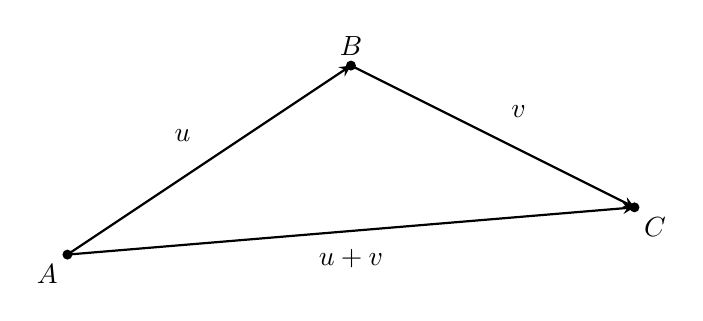
\begin{tikzpicture}[scale=1.2, >=stealth]
			% Pontos
			\coordinate (A) at (0,0);
			\coordinate (B) at (3,2);
			\coordinate (C) at (6,0.5);
			
			% Lados com setas
			\draw[thick, ->] (A) -- (B) node[midway, above left=3pt] {$u$};
			\draw[thick, ->] (B) -- (C) node[midway, above right=3pt] {$v$};
			\draw[thick, ->] (A) -- (C) node[midway, below=3pt] {$u+v$};
			
			% Pontos marcados
			\fill (A) circle (1.5pt) node[below left] {$A$};
			\fill (B) circle (1.5pt) node[above] {$B$};
			\fill (C) circle (1.5pt) node[below right] {$C$};
		\end{tikzpicture}
		(Exemplo no $\mathbb{R}^2$)
		\end{center}
		\end{exemplo}
		\begin{exemplo}[Exemplo de espaço vetorial]
			O conjunto das matrizes $n\times m$ com soma entre vetores e multiplicação por escalar definido da seguinte forma:
			\begin{description}
					\item \[
					\begin{bmatrix}
						a_{11} & a_{12} & ... & a_{1m}  \\
						a_{21} & a_{22} & ... & a_{2m} \\
						... & ... & ... & ... \\
						a_{n1} & a_{n2} & ... & a_{nm}
					\end{bmatrix} + \begin{bmatrix}
					b_{11} & b_{12} & ... & b_{1m}  \\
					b_{21} & b_{22} & ... & b_{2m} \\
					... & ... & ... & ... \\
					b_{n1} & b_{n2} & ... & b_{nm}
					\end{bmatrix} = \begin{bmatrix}
					(a+b)_{11} & (a+b)_{12} & ... & (a+b)_{1m}  \\
					(a+b)_{21} & (a+b)_{22} & ... & (a+b)_{2m} \\
					... & ... & ... & ... \\
					(a+b)_{n1} & (a+b)_{n2} & ... & (a+b)_{nm}
					\end{bmatrix}
					\]
					\item \[\alpha \begin{bmatrix}
						a_{11} & a_{12} & ... & a_{1m}  \\
						a_{21} & a_{22} & ... & a_{2m} \\
						... & ... & ... & ... \\
						a_{n1} & a_{n2} & ... & a_{nm}
					\end{bmatrix} = \begin{bmatrix}
					(\alpha a)_{11} & (\alpha a)_{12} & ... & (\alpha a)_{1m}  \\
					(\alpha a)_{21} & (\alpha a)_{22} & ... & (\alpha a)_{2m} \\
					... & ... & ... & ... \\
					(\alpha a)_{n1} & (\alpha a)_{n2} & ... & (\alpha a)_{nm}
					\end{bmatrix}
					\]
			\end{description}
			é um espaço vetorial, chamado de espaço vetorial da matrizes $n\times m$.
		\end{exemplo} \bigskip
		{\Large\textbf{Exercícios}}
		\begin{enumerate}
			\item Descreva o vetor nulo dos seguintes espaços vetoriais, considerando as operações usuais: \hfill 
			\begin{center}
				a)$\mathbb{R}^5$ \hspace{4cm} b)$\mathbb{M}_{3\times 2}$ \hspace{4cm}
			\end{center}
			\item Mostre que o espaço $\mathbb{P}_n = p(x) = a_0 + a_1 x + a_2 x^2 + ... + a_n x^n : a_0, a_1, a_2, a_3, ..., a_n \in \mathbb{R}$ dos
			polinômios reais de grau menor ou igual a $n$ é um espaço vetorial real, com as operações usuais de soma e multiplicação por escalar.
			\item Verifique se $V = {x \in \mathbb{R}: x > 0}$ é um espaço vetorial com as operações de adição ($\oplus$) e a multiplicação por escalar ($\odot$) dadas abaixo. Em caso positivo, prove e indique o vetor nulo (neutro aditivo) e o inverso aditivo.
			\begin{center}
				$x \oplus y = xy$ \hspace{1cm} e \hspace{1cm} $\alpha \cdot x = x^\alpha$
			\end{center}
		\end{enumerate} 
		\newpage
	\section{Subespaços Vetoriais}
		Subespaços vetoriais são subconjuntos de um espaço vetorial maior que ainda utilizam das mesmas operações e são ''independentes'' do espaço vetorial original, sendo mais exato:
		\begin{definicao}
			Seja $E$ um espaço vetorial. Um \azul{subespaço vetorial} (ou simplesmente \azul{subespaço}) de $E$ é um subconjunto $F \subset E$ com as seguintes propriedades:
				\begin{enumerate}
				\item[(P1)] $\vec{0} \in F$;
				\item[(P2)] Se $u, v \in F$ então $u+v \in F$;
				\item[(P3)] Se $v \in F$ então, para todo $\alpha \in \mathbb{R}$, $\alpha v \in F$.
			\end{enumerate}
		\end{definicao}
		Decorrendo da definição, percebemos que todo subespaço é um espaço vetorial em si mesmo, também percebemos que em todo espaço vetorial existe o \azul{subespaço trivial}, composto somente pelo vetor nulo.\\ \bigskip
		
		{\Large\textbf{Exercícios}}
		\begin{enumerate}
				\item Prove que um plano é um subespaço vetorial de $\mathbb{R}^3$ se, e somente se, o plano passa pela origem.
				\item Sejam $A_{m\times n}$ e $B_{n \times 1}$ matrizes. Prove que o conjunto solução de $AX = B$ é subespaço vetorial de $M_{n\times 1}$ se, e somente se, $B = 0$.
		\end{enumerate}
	
	\section{Base e Coordenadas}
	
	
	
	\section{Ortogonalidade}
		\subsection{Processo de Ortogonalização de Gram-Schmidt}
	
\end{document}
